%!TEX root=../document.tex

% Pierre
\section{Lustre}
Lustre, eine sprachliche Kombination aus den Wörtern ''Linux'' und ''Cluster'', ist besonders für sehr große Systeme mit großen Mengen an Dateien konzipiert. Dabei können Systeme mit Datenmengen über \textbf{100 petabyte} unterstützt werden, mit einem Datenfluss über \textbf{mehrere gigabyte pro Sekunde}. \cite{Lustrea}

Es ist POSIX-konform und läuft allen Linux Betriebssysteme. Wie schon bereits erwähnt, hebt sich Lustre vor allem darin von anderen verteilen Dateisysteme davon ab, dass es unabhängig von Hardware-Einschränken den Speicher und Performance problemlos skalieren kann. \cite{Lustreb}

Wichtig ist auch noch, dass Metadaten auf anderen Servern gespeichert werden, um für jeweils verschiedene Arbeitsauslastung optimiert werde zu können:

\begin{minipage}{\linewidth}
	\centering
	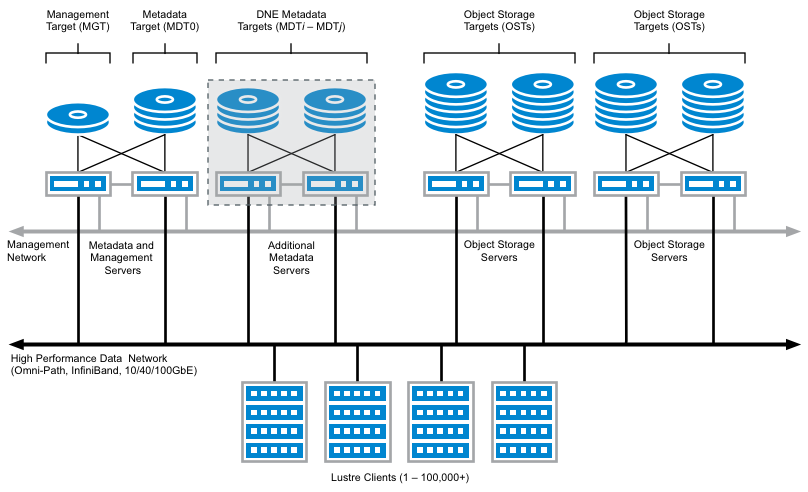
\includegraphics[width=0.8\linewidth]{images/architektur.png}
	\figcaption{Lustre File System Architecture}
\end{minipage}

% Martin
\section{XtreemFS}
XtreemFS ist ebenfalls ein Dateisystem, welches aber nicht nur verteile Dateisysteme unterstützt, sondern ''general purpose''. Es wird keine besondere Hardware oder Software-Kernels benötigt, und es läuft auf Linux, Windows und MAC OS. Im Gegensatz dazu, läuft Lustre nativ nur auf Linux Distributions, bzw. wird ein eigenes Projekt benötigt welches Lustre in Windows portiert. Zusätzlich ist es ebenfalls ''fault-tolerant'' und stark skalierbar. \cite{XtreemFS}

Was nun XtreemFS von anderen verteilten Dateisystemen stark unterscheidet, ist der Fakt dass es dafür entwickelt wurde in ''Wide-Area-Networks'' eingesetzt zu werden, d.h. es ist überall mount-bar und überall zugänglich, auch in sehr großen Netzen. Zusätzlich sind noch Sicherheitsmaßnahmen gegeben, welche sicherstellen, dass wenn über das Netz verteilt wird, auch alle Pakete sicher, vertraulich und \textbf{komplett} ankommen. Dies wurde Umgesetzt mit verschiedenen \textbf{RAID-Konfigurationen} sowie stetig überwachte Prüfsummen. Dies führt zu einem System, welches weniger anfällig auf Serverausfälle bzw. Server-downtime ist. \cite{XtreemFSa}


% Martin
\section{Ceph}
Der Source-code für Ceph ist für jeden Entwickler einsichtbar und nur durch die Community wurde Ceph zu dem, was es heute ist. Das System arbeitet mit Objektspeicherung, welches wieder REST interfaces verwendet um mit vielen Applikationen kompatibel zu sein. Besonders mit S3 und Swift funktioniert Ceph einwandfrei. Zusätzlich wird mit der ''Block-Storage'' Technik gearbeitet, welche im Endeffekt die Daten welche gespeichert werden soll in Blöcke aufteilt auf welche zugegriffen werden kann. Zusätzlich wird wie bei den anderen Systemen ein POSIX-komformes Dateisystem angeboten, mit welchem hohe Leistung, viel Speicher und leichte Skalierung versprochen wird.\cite{Ceph}

Ein Problem bei Ceph besteht darin, im Vergleich zu den anderen verteilten Dateisystemen ist, dass es nicht in einer Docker-Umgebung verwendet werden kann, dafür müsste CephFS verwendet werden, welche noch nicht ausgereift ist. \cite{Feriante}

Ein klarer Vorteil an Ceph ist, dass es den sogenannten \textbf{CRUSH-Algorithmus} verwendet. Dies bedeutet, dass kein zentraler Metadata Service gebraucht wird um Daten zu lokalisieren. Nachteil allerdings an dieser Vorgehensweise, ist das Daten herumgeschoben werden damit der CRUSH-Algorithmus funktioniert. \cite{Yehorov}
